\documentclass[tikz,border=10pt]{standalone}
\begin{document}
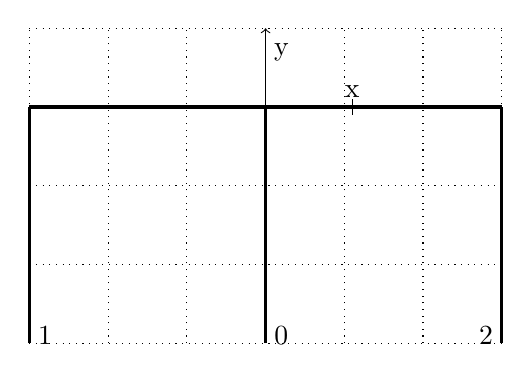
\begin{tikzpicture}
\draw[thin,dotted] (-3,-3) grid (3,1);
\draw[->] (0,0) -- (0,1);
\node at (0.2,0.7)  {y};
\draw[very thick] (-3,0) -- (3,0);
\draw[very thick] (-3,-3) -- (-3,0);
\draw[very thick] (3,-3) -- (3,0);
\draw[very thick] (0,-3) -- (0,0);
\draw (1.1,-0.1) -- (1.1,0.1);
\node at (1.1,0.2) {x};
\node at (-2.8,-2.9) {1};
\node at (0.2,-2.9) {0};
\node at (2.8,-2.9) {2};
\end{tikzpicture}
\begin{itemize}
   \item first;
       \item second.
\end{itemize}
\begin{enumerate}
   \item one;
       \item two;
           \item three.
\end{enumerate} 

\begin{description}
    \item [aaaa] one;
    \item [bbb] two.
\end{description}
abracadabra \footnote{ cccccc}
\end{document}

